\begin{center}
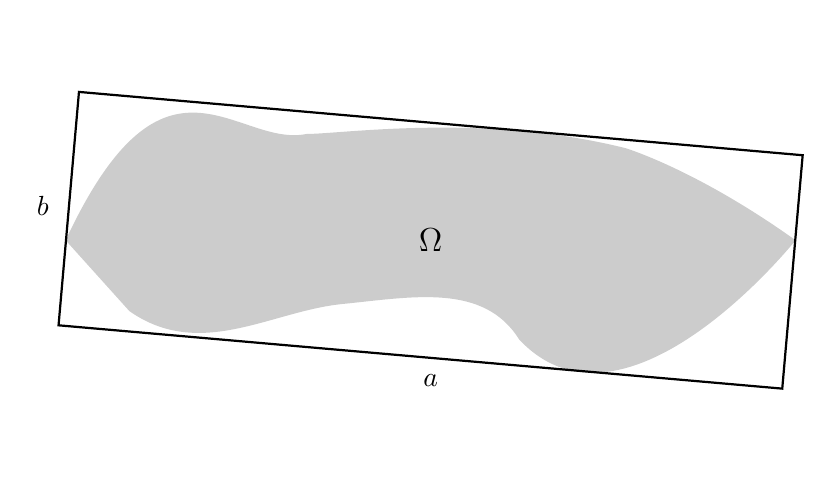
\begin{tikzpicture}[scale=0.9]
    \fill[gray!50, opacity=0.8]
        % Start point (bottom leftish)
        (-.4, 0) .. controls (1, 3) and (2, 1.3) .. (3, 1.5)
        .. controls (3.5, 1.5) and (5.5, 1.8) .. (7.5, 1.3)
        .. controls (7.5, 1.3) and (8.5, 1) .. (9.9, 0) % Top right bump
        .. controls (9.9, 0) and (7.5, -3) .. (6, -1.4)
        .. controls (5.5, -0.6) and (4.5, -0.8) .. (3.5, -0.9)
        .. controls (2.5, -1) and (1.5, -1.7) .. (0.5, -1) -- cycle; % Close the path

    % Draw the label G in the center of the filled region
    \node[label={[font=\large, text=black]center:{$\Omega$}}] at (4.75, 0) {};

    % Now, let's draw the bounding box around this region.
    % We'll estimate the min/max x and y based on the coordinates used above.
    % For a rotated bounding box, it's a bit trickier than an axis-aligned one.
    % To replicate the image, we'll draw a rectangle and then rotate it.
    % This is an illustrative bounding box, not necessarily the *minimal* one calculated from the path.

    % Define bounding box corners relative to the elongated shape.
    % This will be rotated.
    \coordinate (BL) at (-0.5,-1.2); % Bottom-Left of the *unrotated* box
    \coordinate (BR) at (10.0,-1.2); % Bottom-Right
    \coordinate (TR) at (10.0,1.2);  % Top-Right
    \coordinate (TL) at (-0.5,1.2);  % Top-Left

    \begin{scope}[rotate around={-5:(4.75,0)}] % Rotate the box around the center of G
        \draw[black, thick] (BL) rectangle (TR);

        % Label sides 'a' and 'b' on the rotated box
        % You'll need to adjust positions slightly based on rotation
        \path (BL) -- (BR) node[midway, below=5mm] (label_a) {$a$};
        \path (BL) -- (TL) node[left, pos=0.7] (label_b) {$b$};
    \end{scope}

\end{tikzpicture}
\end{center}